% !TeX root = ../main.tex
% Add the above to each chapter to make compiling the PDF easier in some editors.
\chapter{Time-Series Generation Tool}\label{chapter:tool}

We have looked in detail at two approaches to generating time-series, first studying their theory, then implementing them in Python. The result of this is a command-line tool for generating time-series \parencite{tsgenerator}. This chapter will discuss its usage. 

\section{General Options}

There are a lot of command-line options available in this tool. We will first go over the general ones. 

\texttt{---method}: On a high level there are four different modes of operation. Three are based on Hidden Markov Models and one on Singular Spectrum Analysis. They are called \texttt{hmm-learn}, \texttt{hmm-param-simple}, \texttt{hmm-param}, and \texttt{ssa}. This option selects which one of them to use. 

\texttt{---length}: All methods can generate time-series of variable length. This option specifies how many samples should be generated. 

\texttt{---output}: The tool will output the time-series in the CSV format. One column will be the time points and the second column will contain the generated values. Using this option you can specify a file to write this CSV data to. If none is specified the data will be printed to stdout. 

\texttt{---time-increment}: This affects the values in the first ``time'' column of the output. By default, the increment is 1, but it can be changed with this option. 

\texttt{---scaling}: For this option you specify two values: a new minimum and a new maximum. After the generation is complete, this applies scaling so that the minimum and maximum values of the generated time-series become the specified ones. 

\texttt{---display}: By default, the time-series is only output in CSV text form. If this option is enabled the tool will display a graph of the generated series as well. This is very helpful for visualization!

\section{Method: hmm-learn}

The first available method is \texttt{hmm-learn}. The idea is to specify training time-series, from which the tool learns HMM parameters that are then used to generate the time-series. This method comes with its own options:

\texttt{---hmm-training}: This is a path to a CSV containing the training data. Each row is considered one individual time-series. 

\texttt{---hmm-components}: This is the number of hidden states to use in the HMM. 

\texttt{---hmm-iterations}: This is the number iterations that the EM-algorithm will be run. This number does not have to be huge since the algorithm usually converges quite quickly. A good range is 10 to 50 iterations.

\texttt{---display}: This will print the current iteration number and the current log-likelihood during every iteration. This can be helpful since depending on the setup the learning step can take quite a while. Moreover, by looking at the log-likelihood you can get a sense of the convergence. 

\begin{figure}
\begin{singlespace}
\begin{lstlisting}[language=Python]
def generate_hmm(startprop, transmat, means, cov, l):
    k = startprop.size
    start = np.random.choice(range(k), p=startprop)
    mu = means[start]
    hiddenstates = [start]
    sigma = np.sqrt(cov[start])
    first_output = np.random.normal(mu, sigma)
    samples = [first_output]
    for _ in range(l-1):
        prevstate = hiddenstates[-1]
        nextstate = np.random.choice(range(k), p=transmat[prevstate])
        hiddenstates += [nextstate]
        mu = means[nextstate]
        sigma = np.sqrt(cov[nextstate])
        next_output = np.random.normal(mu, sigma)
        samples += [next_output]
    return samples
\end{lstlisting}
\end{singlespace}
\caption{HMM Function: generate\_hmm}    
\label{fig:hmm-generate}
\end{figure}

We have looked at the implementation of the parameter learning using the Baum-Welch algorithm in detail. However, we have not looked at the actual time-series generation code. The implementation from the tool is listed in Figure \ref{fig:hmm-generate}. 

The idea is to generate a hidden state sequence based on the start and transition probabilities. For this \texttt{np.random.choice} from numpy is used, which allows drawing from a set with a given probability vector $p$. From the hidden states we obtain the corresponding means and variances and draw the data points from a normal distribution using \texttt{np.random.normal}.

\section{Method: hmm-param}

This method works by specifying the HMM parameters manually instead of learning them from training data. This method offers the following options: 

\texttt{---hmm-means}: This is the means $\mu$ parameter in a semi-continuous HMM. 

\texttt{---hmm-cov}: This is the variance $\sigma$ parameter in a semi-continuous HMM. 

\texttt{---hmm-start-prop}: This is the start probability parameter $\pi$ in an HMM. 

\texttt{---hmm-trans-prop}: This is the transition probability parameter $a$ in an HMM. 

Note that the dimensions of these parameters have to match up. \texttt{hmm-means}, \texttt{hmm-cov}, and \texttt{hmm-start-prop} all need to have the same length $k$, while \texttt{hmm-trans-prop} needs to be the square of that: $k^2$. 

\section{Method: hmm-simple-param}

This tool already requires a lot of command-line options to be specified. However, in the \texttt{hmm-param} method this becomes unreasonable. This is why the \texttt{hmm-simple-param} method exists, where you only have to specify the means: 

\texttt{---hmm-means}: This is the means $\mu$ parameter in a semi-continuous HMM. 

The rest of the parameters the tool will pick automatically. All variences will be 20\% of the covariance of the means vector. The start probabilities will be evenly distributed. The transition probabilities are also evenly distributed, but with a bias towards staying in the same state. 

As an example consider that the following means vector was given: 

\begin{equation}
    \mu = (10, 30, 40, 70)^T
\end{equation}

The remaining parameters will be chosen in this way:

\begin{equation}
    \begin{split}
    a = 
    \begin{pmatrix}
        0.625 & 0.125 & 0.125 & 0.125 \\
        0.125 & 0.625 & 0.125 & 0.125 \\
        0.125 & 0.125 & 0.625 & 0.125 \\
        0.125 & 0.125 & 0.125 & 0.625
    \end{pmatrix} \\
    \sigma^2 = (144, 144, 144, 144)^T \\
    \pi = (0.25, 0.25, 0.25, 0.25)^T 
\end{split}
\end{equation}

\section{Method: ssa}

The last method of generating is Singular Spectrum Analysis forecasting. This also offers some command-line options: 

\texttt{---ssa-original}: This points towards a CSV file with the time-series that is to be forecasted. 

\texttt{---ssa-window}: This is the window length for the SSA embedding. The window length should not be too small but also not larger than $N/2$, where $N$ is the length of the original series. Moreover, the window length should be a multiple of any suspected seasonality.

\texttt{---ssa-components}: This is the number of eigentriple components to use in the time-series approximation and the recurrence forecasting. Smaller values will lead to a smoother approximation, while large ones make the approximation more accurate. 

\section{Examples}

\begin{figure}
\begin{lstlisting}[language=bash]
    python generate.py --method hmm-learn \
    --hmm-training wikipedia-overall-2019-list.csv --hmm-components 4 \
    --hmm-iterations 10 --show-progress --length 20 --display
\end{lstlisting}
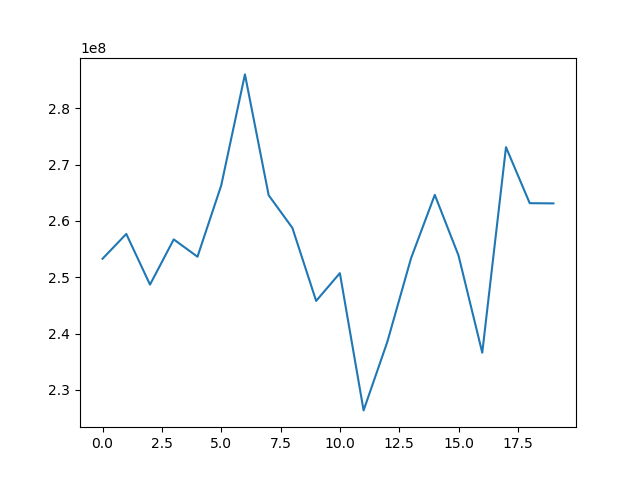
\includegraphics[scale=0.7]{figures/hmm-learn}
\caption{Example: hmm-learn}    
\label{fig:hmm-learn-example}
\end{figure}

Figure \ref{fig:hmm-learn-example} shows an example of the usage of the \texttt{hmm-learn} method. The specified training data is a time-series of daily page views of Wikipedia in 2019 \parencite{wikipedia}.

\newpage

\begin{figure}
\begin{lstlisting}[language=bash]
    python generate.py --method hmm-param-simple --length 20 \
    --hmm-simple-means 10 30 40 70 --display
\end{lstlisting}
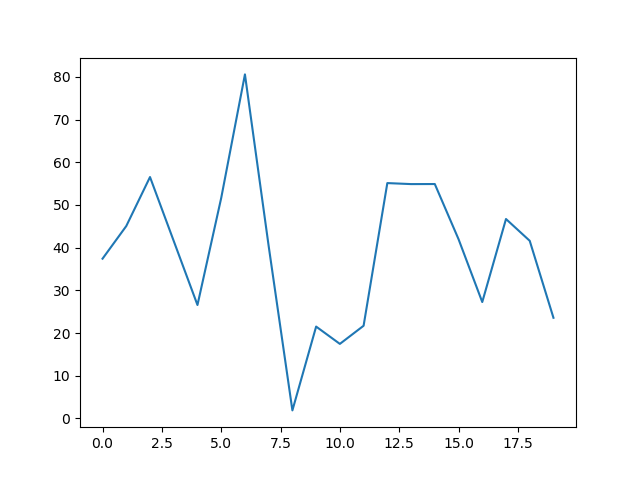
\includegraphics[scale=0.7]{figures/hmm-param-simple}
\caption{Example: hmm-param-simple}    
\label{fig:hmm-param-simple-example}
\end{figure}

Figure \ref{fig:hmm-param-simple-example} shows an example of the usage of the \texttt{hmm-param-simple} method. It uses the previously discussed example $\mu = (10, 30, 40, 70)^T$. 

\newpage

\begin{figure}
\begin{lstlisting}[language=bash]
    python generate.py --method hmm-param --length 20 \
    --hmm-means 10 30 40 70 --hmm-cov 144 144 144 144 \
    --hmm-start-prop 0.25 0.25 0.25 0.25 --hmm-trans-prop \
    0.625 0.125 0.125 0.125 0.125 0.625 0.125 0.125 0.125 \
    0.125 0.625 0.125 0.125 0.125 0.125 0.625 --display
\end{lstlisting}
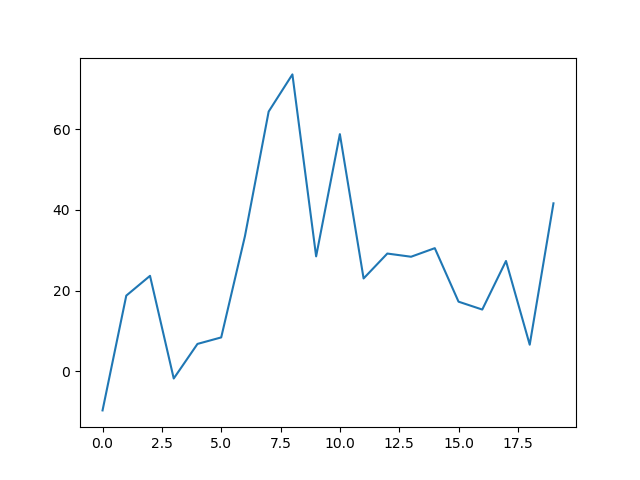
\includegraphics[scale=0.7]{figures/hmm-param}
\caption{Example: hmm-param}    
\label{fig:hmm-param-example}
\end{figure}

Figure \ref{fig:hmm-param-example} uses the same parameters as Figure \ref{fig:hmm-param-simple-example}, but with all the parameters spelled out manually using the \texttt{hmm-param} method. 

\newpage

\begin{figure}
\begin{lstlisting}[language=bash]
    python generate.py --method ssa --length 170 --ssa-original \
    airpassenger-list.csv --ssa-window 36 --ssa-components 13 --display
\end{lstlisting}
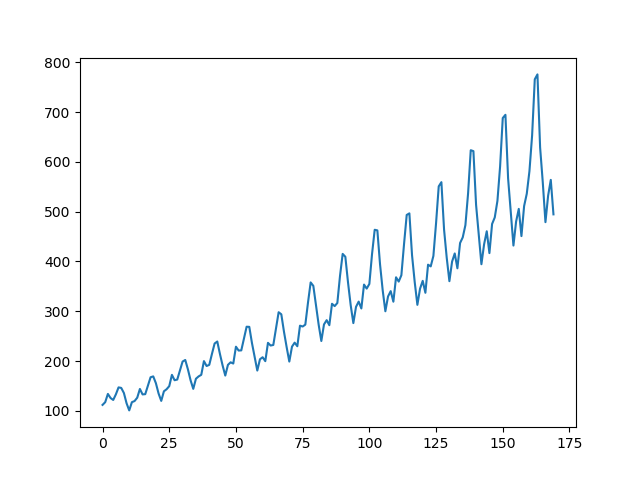
\includegraphics[scale=0.7]{figures/ssa}
\caption{Example: ssa}    
\label{fig:ssa-example}
\end{figure}

Figure \ref{fig:ssa-example} is an example of the \texttt{ssa} method. The data is airplane passenger data per month in the US. This is an ideal time-series for SSA since there are clear trend and seasonality. The original time-series is 144 long, so the values past that are forecasted.